前節までは、比較的単純なサンプルコードを用いて、FDPSの基本的な機能について解説を行ってきた。しかしながら、実際の研究では、複数の粒子種の取り扱いが必要になる等、より複雑なアプリケーションを書く必要がある。そこで、本節では、より実用的なサンプルコードを使って、FDPSの他の機能について解説を行う。\ul{記述を簡潔にするため、読者は前節までの内容を理解しているものと仮定する}。
%=============================
%   N-body+SPH コードの解説
%=============================
\subsection{$N$体/SPHコード} \label{subsec:NbodySPH}
本節では、より実用的なアプリケーションの一例として円盤銀河の時間発展を計算する$N$体/SPHサンプルコードの解説を行う。このサンプルコードは、重力のみで相互作用するダークマターと星を$N$体粒子、重力及び流体相互作用を行うガスをSPH粒子として表現する。重力計算はTree法で、流体計算はSPH法を用いて行う。SPH法は\href{https://doi.org/10.1046/j.1365-8711.2002.05445.x}{Springel \& Hernquist [2002, MNRAS, 333, 649]}及び\href{https://doi.org/10.1111/j.1365-2966.2005.09655.x}{Springel [2005, MNRAS, 364, 1105]}で提案された方法(以下、簡単のため、Springelの方法と呼ぶ)を使用している。本解説を読むことにより、ユーザは、FDPSで複数の粒子種を扱う方法を学ぶことができる。

以下では、まずはじめにコードの使用方法について説明を行う。次にSpringelの方法について簡単な解説を行った後、サンプルコードの中身について具体的に解説する。

\subsubsection{コードの使用方法}
\label{subsubsec:NbodySPH_usage}
前節で述べた通り、本コードは円盤銀河の$N$体/SPHシミュレーションを行うコードである。ダークマターと星の初期条件は、銀河の初期条件を作成するソフトウェア\href{https://bitbucket.org/ymiki/magi}{\textsc{MAGI}} (\href{https://doi.org/10.1093/mnras/stx3327}{Miki \& Umemura [2018, MNRAS, 475, 2269]})で作成したファイルを読み込んで設定する。一方、ガスの初期条件は本コードの内部で作成する。したがって、以下の手順で本コードを使用する。
\begin{itemize}
\item ディレクトリ\dirNameNbodySPHSample に移動
\item カレントディレクトリにある\texttt{Makefile}を編集
\item \href{https://bitbucket.org/ymiki/magi}{\textsc{MAGI}}を使って初期条件に対応する粒子データを生成し、\texttt{./magi\_data/dat}以下に配置
\item コマンドライン上で\texttt{make}を実行
\item \texttt{nbodysph.out}ファイルの実行
\item 結果の解析
\end{itemize}

以下、順に説明していく。

\subsubsubsection{ディレクトリ移動}
\label{s3sec:NbosySPH_code_loc}
サンプルコードの場所は、\dirNameNbodySPHSample である。まずは、そこに移動する。

\subsubsubsection{サンプルコードのファイル構成}
\label{s3sec:NbodySPH_file_str}
以下はサンプルコードのファイル構成である。
\ifCpp %C++用
\begin{screen}
\begin{verbatim}
$ ls | awk '{print $0}'
Makefile
Makefile.K
Makefile.ofp
ic.hpp
job.K.sh
job.ofp.sh
leapfrog.hpp
macro_defs.hpp
magi_data/
main.cpp
mathematical_constants.cpp
mathematical_constants.h
physical_constants.cpp
physical_constants.h
test.py*
user_defined.hpp
\end{verbatim}
\end{screen}
各ソースファイルの内容について簡単に解説を行う。まず、\texttt{ic.hpp}には初期条件を作成する関数が実装されている。初期条件は円盤銀河の他、複数用意されている(後述)。\texttt{leapfrog.hpp}には粒子の軌道の時間積分をLeapfrog法を用いて行う関数が実装されている。\texttt{macro\_defs.hpp}には計算を制御するためのマクロが定義されている。\texttt{main.cpp}はアプリケーションのメインルーチンが実装されている。\texttt{mathematical\_constants.h}及び\texttt{mathematical\_constants.cpp}には数学定数が、\texttt{physical\_constants.h}及び\texttt{physical\_constants.cpp}には物理定数が定義されている。\texttt{user\_defined.hpp}には、ユーザ定義クラスや相互作用関数が実装されている。
\endifCpp
\ifFtn %Fortran用
\begin{screen}
\begin{verbatim}
$ ls | awk '{print $0}'
Makefile
Makefile.K
Makefile.intel
Makefile.ofp
f_main.F90
ic.F90
job.K.sh
job.ofp.sh
leapfrog.F90
macro_defs.h
magi_data/
mathematical_constants.F90
physical_constants.F90
test.py
tipsy_file_reader.cpp
tipsy_file_reader.h
user_defined.F90
\end{verbatim}
\end{screen}
各ソースファイルの内容について簡単に解説を行う。まず、\texttt{ic.F90}には初期条件を作成するサブルーチンが実装されている。初期条件は円盤銀河の他、複数用意されている(後述)。\texttt{leapfrog.F90}には粒子の軌道の時間積分をLeapfrog法を用いて行うサブルーチンが実装されている。\texttt{macro\_defs.h}には計算を制御するためのマクロが定義されている。\texttt{f\_main.F90}はアプリケーションのメインルーチンが実装されている。\texttt{mathematical\_constants.F90}には数学定数が、\texttt{physical\_constants.F90}には物理定数が定義されている。\texttt{tipsy\_file\_reader.cpp} 及び \texttt{tipsy\_file\_reader.h} には\textsc{MAGI}が出力した粒子データを読むための関数が定義されている。\texttt{user\_defined.F90}には、ユーザ定義型や相互作用関数が実装されている。
\endifFtn
\ifC %C用
\begin{screen}
\begin{verbatim}
$ ls | awk '{print $0}'
Makefile
Makefile.ofp
c_main.c
ic.c
ic.h
job.ofp.sh
leapfrog.c
leapfrog.h
macro_defs.h
magi_data/
mathematical_constants.c
mathematical_constants.h
physical_constants.c
physical_constants.h
tipsy_file_reader.cpp
tipsy_file_reader.h
user_defined.c
user_defined.h
\end{verbatim}
\end{screen}
各ソースファイルの内容について簡単に解説を行う。まず、\texttt{c\_main.c}はアプリケーションのメイン関数が実装されている。\texttt{ic.*}には初期条件を作成する関数が実装されている。初期条件は円盤銀河の他、複数用意されている(後述)。\texttt{leapfrog.*}には粒子の軌道の時間積分をLeapfrog法を用いて行う関数が実装されている。\texttt{macro\_defs.h}には計算を制御するためのマクロが定義されている。\texttt{mathematical\_constants.*}には数学定数が、\texttt{physical\_constants.*}には物理定数が定義されている。\texttt{tipsy\_file\_reader.*}には\textsc{MAGI}が出力した粒子データを読むための関数が定義されている。\texttt{user\_defined.*}には、ユーザ定義型や相互作用関数が実装されている。
\endifC


ディレクトリ\texttt{magi\_data}には、銀河の初期条件を作成するソフトウェア\textsc{MAGI}に入力するパラメータファイル(\texttt{magi\_data/cfg/*})と\textsc{MAGI}を動作させるスクリプト(\texttt{magi\_data/sh/run.sh})が格納されている。

\subsubsubsection{Makefileの編集}
\label{s3sec:NbodySPH_Makefile}
\path{Makefile}の編集項目は以下の通りである。
\begin{itemize}
\item 変数\path{CXX}に使用するC++コンパイラを代入する。
\ifFtn %Fortran用
\item 変数\path{FC}に使用するFortranコンパイラを代入する。
\endifFtn
\ifC %C言語用
\item 変数\path{CC}に使用するCコンパイラを代入する。
\endifC
\item 変数\path{CXXFLAGS}にC++コンパイラのコンパイルオプションを指定する。
\ifFtn %Fortran用
\item 変数\path{FCFLAGS}にFortranコンパイラのコンパイルオプションを指定する。
\endifFtn
\ifC %C言語用
\item 変数\path{CFLAGS}にCコンパイラのコンパイルオプションを指定する。
\endifC
\item 本コードでは計算を制御するためにいくつかのマクロを用意している。表\ref{tbl:NbodySPH:compile_time_macros}にマクロ名とその定義の対応を示した。また、本コードには、\path{INITIAL_CONDITION}の値に応じて自動的に設定されて使用されるマクロも存在する。これらは一般に変更する必要はないが、詳細は\path{macro_defs.h}を参照して頂きたい。
\item 本コードでは重力計算にx86版Phantom-GRAPEライブラリを使用することができる。Phantom-GRAPEライブラリを使用する場合、\path{Makefile}の変数\path{use_phantom_grape_x86}の値を\path{yes}にする。
\end{itemize}
OpenMPやMPIの使用/不使用の指定に関しては、第\ref{sec:getting_started}節を参照して頂きたい。

\begin{table}[H]
\begin{tabularx}{\linewidth}{|c|X|}
\toprule
\rowcolor{Snow2}
マクロ名 & 定義 \\
\midrule
\path{INITIAL_CONDITION} & 初期条件の種類の指定、或いは、コードの動作の指定に使用されるマクロ。0から3までのいずれかの値を取る必要がある。値に応じて、次のように指定される。 0:円盤銀河の初期条件を選択、1:Cold collapse 問題の初期条件を選択、2:Evrard test 問題の初期条件を選択、3:ガラス状に分布したSPH粒子データを生成するモードで実行ファイルを作成 \\
\midrule
\path{ENABLE_VARIABLE_SMOOTHING_LENGTH} & smoothing lengthが可変/固定を制御するマクロ。定義されている場合、可変となりSpringelの方法でSPH計算が行われる。未定義の場合、固定長カーネルのSPHコードとなる。 \\
\midrule
\path{USE_ENTROPY} & 流体の熱力学状態を記述する独立変数としてエントロピーを使うか単位質量あたりの内部エネルギーを使用するかを指定するマクロ。定義されている場合エントロピーが用いられる。但し、後述するマクロ\path{ISOTHERMAL_EOS}が定義されている場合には、単位質量あたりの内部エネルギーが強制的に使用される(圧力の計算に内部エネルギーを使用する)。 \\
\midrule
\path{USE_BALSARA_SWITCH} & Balsara switch (\href{https://doi.org/10.1016/S0021-9991(95)90221-X}{Balsara [1995, JCP, 121, 357]})の使用/不使用を制御するマクロ。定義されている場合は使用する。 \\ 
\midrule
\path{USE_PRESCR_OF_THOMAS_COUCHMAN_1992} & \href{https://doi.org/10.1093/mnras/257.1.11}{Thomas \& Couchman [1992, MNRAS,257, 11]}で提案されたSPH計算のtensile不安定を防ぐ簡便な方法を使用するかを制御するマクロ。定義されている場合は使用する。\\
\midrule
\path{ISOTHERMAL_EOS} & 流体を等温で取り扱うかどうかを指定するマクロ。定義されている場合は等温で扱い、未定義の場合にはエントロピー方程式、或いは、内部エネルギー方程式が解いて、熱力学的状態を時間発展させる。\\
\midrule
\path{READ_DATA_WITH_BYTESWAP} & \textsc{MAGI}の粒子データを読み込む際に基本データ型単位でbyteswapしてデータを読み込むかを制御するマクロ。定義されている場合はbyteswapする。\\
\bottomrule
\end{tabularx}
\caption{コンパイル時マクロの種類と定義}
\label{tbl:NbodySPH:compile_time_macros}
\end{table}

\subsubsubsection{MAGIを使った粒子データの生成}
\label{s3sec:NbodySPH_MAGI_usage}
前述した通り、ユーザは事前に銀河の初期条件を作成するソフトウェア\textsc{MAGI}を使い、以下に指定する手順でデータを作成する必要がある。\textsc{MAGI}を利用できないユーザは、指定するサイトからこちらが用意したデータをダウンロードすることも可能である。以下、各場合について詳しく述べる。
\begin{description}
\item[\textsc{MAGI}を使ってデータ作成を行う場合] 以下の手順でデータ作成を行う。
\begin{enumerate}
\item \href{https://bitbucket.org/ymiki/magi}{https://bitbucket.org{\slash}ymiki{\slash}magi}から\textsc{MAGI}をダウンロードし、Webの``How to compile MAGI"に記載された手順に従って、適当な場所にインストールする。但し、本サンプルコードはTIPSYファイルの粒子データ読み込みしかサポートしていないため、MAGIは\path{USE_TIPSY_FORMAT=ON}の状態でビルドされている必要がある。
\item \texttt{./magi\_data/sh/run.sh}を開き、変数\texttt{MAGI\_INSTALL\_DIR}にコマンド\texttt{magi}がインストールされたディレクトリを、変数$\texttt{NTOT}$に希望する$N$体粒子の総数をセットする(ダークマターと星への振り分けは\textsc{MAGI}が自動的に行う)。
\item \texttt{./magi\_data/cfg/*}を編集し、ダークマターと銀河のモデルを指定する。指定方法の詳細は上記サイトか、或いは、\href{https://doi.org/10.1093/mnras/stx3327}{Miki \& Umemura [2018, MNRAS, 475, 2269]}の第2.4節を参照のこと。デフォルトの銀河モデル(以下、\textbf{デフォルトモデル})は次の4成分から構成される:
\begin{enumerate}[label=(\roman*)]
\item ダークマターハロー (NFW profile, $M=10^{12}\;\mathrm{M_{\odot}}$, $r_{s}=21.5\;\mathrm{kpc}$, $r_{c}=200\;\mathrm{kpc}$, $\Delta_{c}=10\;\mathrm{kpc}$)
\item バルジ (Kingモデル, $M=5\times 10^{10}\;\mathrm{M_{\odot}}$, $r_{s}=0.7\;\mathrm{kpc}$, $W_{0}=5$)
\item thick disk  (S{\'e}rsic profile, $M=2.5\times 10^{10}\;\mathrm{M_{\odot}}$, $r_{s}=3.5\;\mathrm{kpc}$, $n=1.5$, $z_{d}=1\;\mathrm{kpc}$, $Q_{T,\min}=1.0$)
\item thin disk (exponential disk, $M=2.5\times 10^{10}\;\mathrm{M_{\odot}}$, $r_{s}=3.5\;\mathrm{kpc}$, $z_{d}=0.5\;\mathrm{kpc}$, $Q_{T,\min}=1.0$)
\end{enumerate}
デフォルトモデルでは、2つの星円盤はbarモードに対してわずかに不安定であるため、弱い棒状構造を持つ渦巻き銀河になることが期待される初期条件となっている。\textsc{MAGI}の最新のリリース(version 1.1.1 [2019年7月19日時点])では、従来のリリースとデフォルトの動作モードが変更されたため、thick disk と thin disk のパラメータ指定の仕方が FDPS 5.0d 以前から変わっていることに注意されたい。具体的には、従来の\textsc{MAGI}では disk 成分の速度分散をパラメータ $f$ を通して指定する形になっていたが(FDPS 5.0d 以前に付属するサンプルコードでは、$f=0.125$)、最新のリリースでは Toomore Q value の最小値 $Q_{T,\min}$ を通して指定する方式になっている。
\item ディレクトリ\texttt{magi\_data}に移動し、以下のコマンドを実行:
\begin{screen}
\$ ./sh/run.sh
\end{screen}
\item \textsc{MAGI}が正しく終了しているなら、\path{magi_data/dat}以下に、拡張子が\texttt{tipsy}の粒子データが生成されているはずである。
\end{enumerate}
\item[データをダウンロードする場合]  以下のサイトからダウンロードし、\texttt{./magi\_data/dat/}以下に置く。各粒子データの銀河モデルはすべてデフォルトモデルで、粒子数だけ異なる。
\begin{itemize}
\item $N=2^{21}$: \url{https://v2.jmlab.jp/owncloud/index.php/s/XnzvW5XAYwfqZYQ/download?path=%2Fmagi_data%2FGalaxy%2F21&files=Galaxy.tipsy}
\item $N=2^{22}$: \url{https://v2.jmlab.jp/owncloud/index.php/s/XnzvW5XAYwfqZYQ/download?path=%2Fmagi_data%2FGalaxy%2F22&files=Galaxy.tipsy}
\item $N=2^{23}$: \url{https://v2.jmlab.jp/owncloud/index.php/s/XnzvW5XAYwfqZYQ/download?path=%2Fmagi_data%2FGalaxy%2F23&files=Galaxy.tipsy}
\item $N=2^{24}$: \url{https://v2.jmlab.jp/owncloud/index.php/s/XnzvW5XAYwfqZYQ/download?path=%2Fmagi_data%2FGalaxy%2F24&files=Galaxy.tipsy}
\end{itemize}
\end{description}

\subsubsubsection{makeの実行}
\label{s3sec:NbodySPH_make}
\path{make}コマンドを実行する。

\subsubsubsection{実行}
\label{s3sec:NbodySPH_execution}
実行方法は以下の通りである。
\begin{itemize}
\item MPIを使用しない場合、コマンドライン上で以下のコマンドを実行する
\begin{screen}
\begin{verbatim}
$ ./nbodysph.out
\end{verbatim}
\end{screen}
  
\item MPIを使用する場合、コマンドライン上で以下のコマンドを実行する
\begin{screen}
\begin{verbatim}
$ MPIRUN -np NPROC ./nbodysph.out
\end{verbatim}
\end{screen}
ここで、\texttt{MPIRUN}には\texttt{mpirun}や\texttt{mpiexec}などが、\texttt{NPROC}には使用するMPIプロセスの数が入る。
\end{itemize}

\subsubsubsection{結果の解析}
\label{s3sec:NbodySPH_result_analysis}
ディレクトリ\path{result}に$N$体粒子とSPH粒子の粒子データファイル
\describeForCpp{%C++用
``nbody0000x.dat"と``sph0000x.dat"が出力される。ここでxは時刻に対応する整数である。
}
\describeForIF{%Fortran,C用
``nbody0000x-proc0000y.dat"と``sph0000x-proc0000y.dat"が出力される。ここでxは時刻に対応する整数、yはMPIのプロセス番号(ランク番号)を表す。
}
$N$体粒子データの出力フォーマットは、1列目から順に粒子のID, 粒子の質量、位置のx, y, z座標、粒子のx, y, z軸方向の速度となっている。一方、SPH粒子データの出力フォーマットは、1列目から順に粒子のID, 粒子の質量、位置のx, y, z座標、粒子のx, y, z軸方向の速度、密度、単位質量あたりの内部エネルギー、エントロピー、圧力となっている。

図\ref{fig:nbodysph}は、$N$体粒子数$2^{21}$、SPH粒子数$2^{18}$で円盤銀河のシミュレーションを行ったときの$T=0.46$における星分布とガス分布である。

% 図の作成
\begin{figure}[h]
\centering
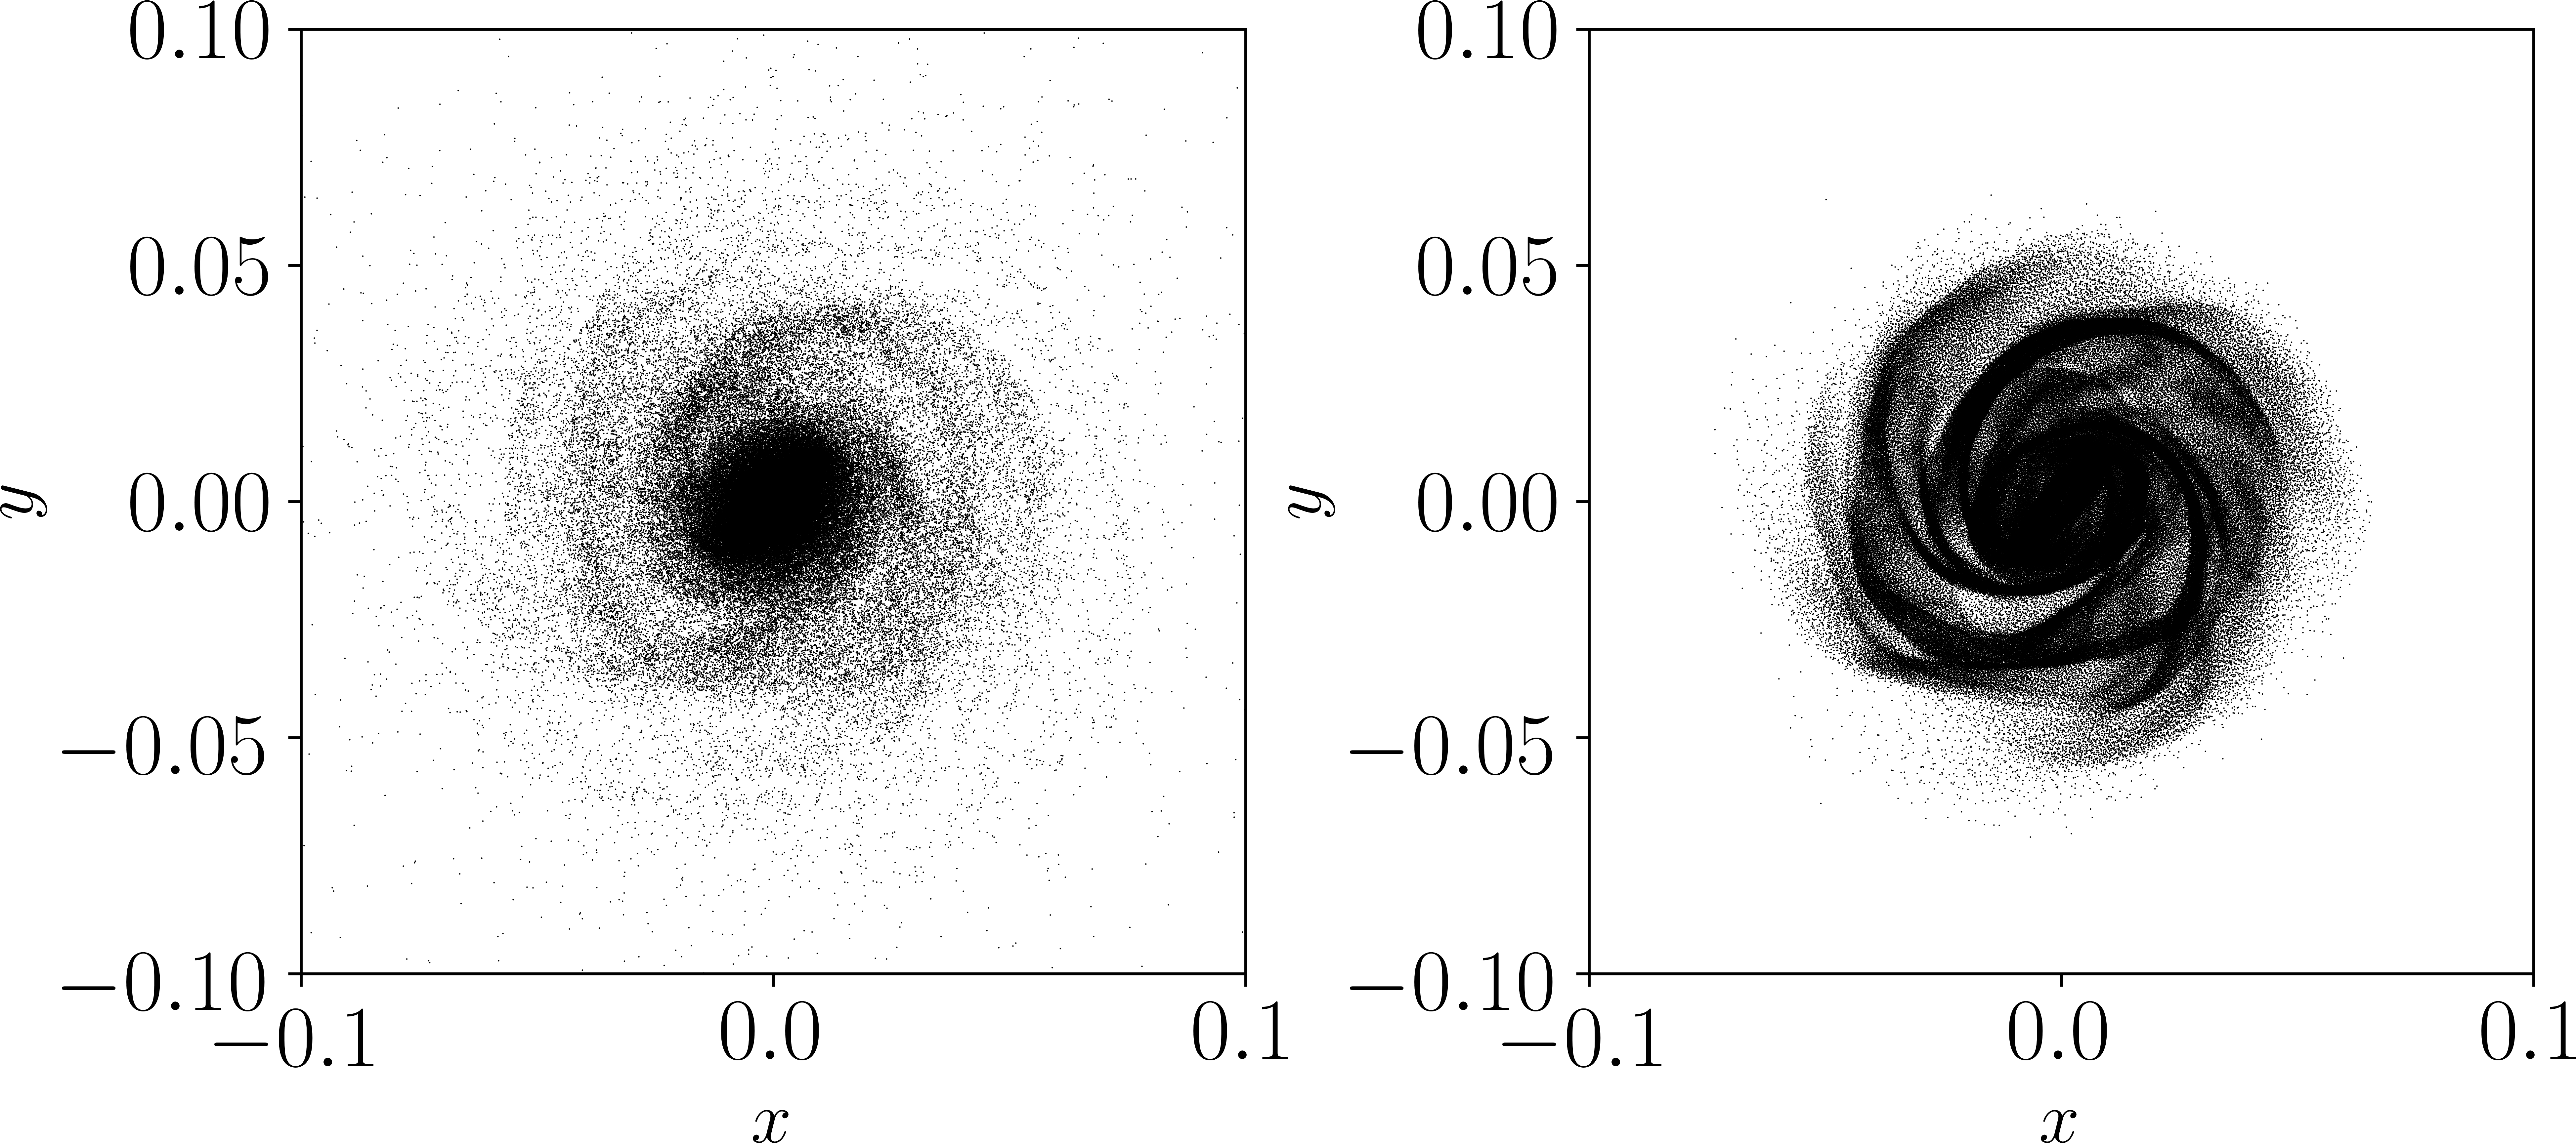
\includegraphics[width=\linewidth]{./fig/nbodysph_t046.png}
\caption{$T=0.46$における星分布(左)とガス分布(右) (計算は以下の条件で実施した: $N$体粒子数$2^{21}$、SPH粒子数$2^{18}$、等温、ガス温度$10^{4}\;\mathrm{K}$、平均分子量$\mu=0.5$)}
\label{fig:nbodysph}
\end{figure}


以下では、まずSpringelの方法について解説し、その後、サンプルコードの実装について説明していく。


\subsubsection{Springelの方法}
\label{subsubsec:Springel_scheme}
\href{https://doi.org/10.1046/j.1365-8711.2002.05445.x}{Springel \& Hernquist [2002, MNRAS, 333, 649]}では、smoothing lengthが可変な場合でも、系のエネルギーとエントロピーが保存するようなスキーム(具体的には運動方程式)を定式化した。以下、彼らの定式化を手短に説明する。導出方針としては、smoothing lengthも独立変数とみて系のLagrangianを立て、それを粒子数個の拘束条件の下、Euler-Lagrange方程式を解く、というものである。

具体的には、彼らは系のLagrangianとして次のようなもの選んだ:
\begin{equation}
L(\bm{q}, \dot{\bm{q}}) = \dfrac{1}{2}\sum^{N}_{i=1}m_{i}\dot{\bm{r}}^{2}_{i} - \dfrac{1}{\gamma -1}\sum^{N}_{i=1}m_{i}A_{i}\rho^{\gamma-1}_{i} \label{eq:Lagrangian}
\end{equation}
ここで、$\bm{q}=(\bm{r}_{1},...,\bm{r}_{N},h_{1},...h_{N})$であり、下付きの整数はすべて粒子番号を表す。$\bm{r}_{i}$は位置、$h_{i}$はsmoothing length、$m_{i}$は質量、$\gamma$は比熱比、$\rho_{i}$は密度、$A_{i}$はエントロピー関数と呼ばれ、単位質量あたりの内部エネルギー$u_{i}$と次の関係がある:
\begin{equation}
u_{i} = \dfrac{A_{i}}{\gamma-1}\rho^{\gamma-1}_{i} \label{eq:relation_between_u_A_rho}
\end{equation}
式(\ref{eq:Lagrangian})の第1項目は運動エネルギー、第2項目は内部エネルギーを表す。このLagrangianをそのままEuler-Lagrangian方程式を使って解くと、$4N$個の方程式になってしまうので、彼らは次の$N$個の拘束条件を導入した。
\begin{equation}
\phi_{i} = \dfrac{4\pi}{3}h^{3}_{i}\rho_{i} - \overline{m}N_{\mathrm{neigh}}=0 \label{eq:Springel_SPH_constraints}
\end{equation}
ここで、$\overline{m}$はSPH粒子の平均質量\footnote{拘束条件に使用していることから、定数扱いであることに注意。}、$N_{\mathrm{neigh}}$は近傍粒子数(定数)である。この拘束条件の下、Lagrangeの未定乗数法を使って、Euler-Lagrange方程式をとけば、以下の運動方程式が得られる:
\begin{equation}
\dfrac{\mathrm{d}\bm{v}_{i}}{\mathrm{d}t} = - \sum^{N}_{j=1}m_{j}\left[f_{i}\dfrac{P_{i}}{\rho^{2}_{i}}\nabla_{i}W(r_{ij},h_{i})+f_{j}\dfrac{P_{j}}{\rho^{2}_{j}}\nabla_{i}W(r_{ij},h_{j})\right] \label{eq:Springel_SPH_EoM_pure_hydro}
\end{equation}
ここで、$P_{i}$は圧力、$r_{ij}=|\bm{r}_{i}-\bm{r}_{j}|$、$W$はカーネル関数、$f_{i}$は$\nabla h$ termと呼ばれる量で、
\begin{equation}
f_{i} = \left(1 + \dfrac{h_{i}}{3\rho_{i}}\dfrac{\partial \rho_{i}}{\partial h_{i}}\right)^{-1} \label{eq:gradh_term}
\end{equation}
と定義される。

系の熱力学的状態はエントロピー$A_{i}$を独立変数として記述される。断熱過程の場合、エントロピーは衝撃波以外のところでは流れに沿って一定である。
\href{https://doi.org/10.1111/j.1365-2966.2005.09655.x}{Springel [2005, MNRAS, 364, 1105]}では、衝撃波でのエントロピー増加と速度の変化を人工粘性を使って次のようにモデル化している:
\begin{align}
\dfrac{\mathrm{d}A_{i}}{\mathrm{d}t} & = \dfrac{1}{2}\dfrac{\gamma-1}{\rho^{\gamma-1}_{i}}\sum^{N}_{j=1}m_{j}\Pi_{ij}\bm{v}_{ij}\cdot\nabla_{i}\overline{W}_{ij} \label{eq:Springel_SPH_entropy_eq} \\
\left.\dfrac{\mathrm{d}\bm{v}_{i}}{\mathrm{d}t}\right|_{\mathrm{visc}} & = -\sum^{N}_{j=1}m_{j}\Pi_{ij}\nabla_{i}\overline{W}_{ij} \label{eq:Springel_SPH_EoM_art_vis}
\end{align}
ここで、$\bm{v}_{ij}=\bm{v}_{i}-\bm{v}_{j}$、$\bm{v}_{i}$は速度、$\overline{W}_{ij}=\frac{1}{2}(W(r_{ij},h_{i})+W(r_{ij},h_{j}))$である。$\Pi_{ij}$に関しては、原論文を参照して頂きたい。

したがって、SPH計算の手順は次のようになる:
\begin{screen}
\begin{enumerate}[leftmargin=*,itemsep=-1ex,label={(\arabic*)}]
\item 式(\ref{eq:Springel_SPH_constraints})と以下の式を無矛盾に解き、密度$\rho_{i}$と$h_{i}$を決定する。
\begin{equation}
\rho_{i} = \sum^{N}_{j=1}m_{j}W(r_{ij},h_{i}) \label{eq:SPH_density_def}
\end{equation}
\item 式(\ref{eq:gradh_term})で定義される$\nabla h$ term を計算する。
\item 式(\ref{eq:Springel_SPH_EoM_pure_hydro})、(\ref{eq:Springel_SPH_entropy_eq})、(\ref{eq:Springel_SPH_EoM_art_vis})の右辺を計算する。
\item SPH粒子の位置、速度、エントロピーを時間積分する。
\end{enumerate}
\end{screen}



以下、まずユーザ定義クラスと相互作用関数の実装について解説を行い、次にメインルーチンの実装について解説を行う。複数粒子種の取扱は後者で解説する。

\subsubsection{ユーザー定義型}
本サンプルコードのユーザ定義型はすべて\describeForEach{\path{user_defined.hpp}}{\path{user_defined.F90}}{\path{user_defined.h}}に定義されている。はじめに用意されているユーザ定義型の種類について簡単に説明しておく。冒頭で述べたように、本サンプルコードは2種類の粒子($N$体粒子, SPH粒子)を扱う。そのため、FullParticle型も2種類用意している($N$体粒子用に\describeForEach{\texttt{FP\_nbody}クラス}{\structure \texttt{fp\_nbody}}{\structure \texttt{fp\_nbody}}を, SPH粒子用に\describeForEach{\texttt{FP\_sph}クラス}{\structure \texttt{fp\_sph}}{\structure \texttt{fp\_sph}})。相互作用は重力相互作用と流体相互作用の2種類ある。そのため、Force型を3種類用意している(重力計算用に\describeForEach{\texttt{Force\_grav}クラス}{\structure \texttt{force\_grav}}{\structure \texttt{force\_grav}}を、密度計算用に\describeForEach{\texttt{Force\_dens}クラス}{\structure \texttt{force\_dens}}{\structure \texttt{force\_dens}}を、そして、圧力勾配による加速度(以下、単に圧力勾配加速度)の計算用に\describeForEach{\texttt{Force\_hydro}クラス}{\structure \texttt{force\_hydro}}{\structure \texttt{force\_hydro}}を; 第\ref{sec:how_to_use}節も参照のこと)。本サンプルコードでは、簡単のため、EssentialParticleI型とEssentialParticleJ型を1つの\structure で兼ねることにし(以下、単にEssentialParticle型)、密度計算と圧力勾配加速度計算に同じEssentialParticle型を使用する。したがって、EssentialParticle型の種類は2種類となっている(重力計算用に\describeForEach{\texttt{EP\_grav}クラス}{\structure \texttt{ep\_grav}}{\structure \texttt{ep\_grav}}を、SPH計算用に\describeForEach{\texttt{EP\_hydro}クラス}{\structure \texttt{ep\_hydro}}{\structure \texttt{ep\_hydro}})。

以下、各ユーザ定義型の実装について説明する。

%--------------------
%   FullParticle型
%--------------------
\subsubsubsection{FullParticle型}
まず、$N$体粒子用のFullParticle型である\describeForEach{\texttt{FP\_nbody}クラス}{\structure \texttt{fp\_nbody}}{\structure \texttt{fp\_nbody}}について解説する。この\structure には、$N$体粒子が持っているべき全ての物理量が含まれている。Listing \ref{nbodysph_FP_nbody}に、この\structure の実装を示す。メンバ変数\describeForCpp{およびメンバ関数}の構成は、第\ref{sec:getting_started}-\ref{sec:how_to_use}節で紹介した$N$体計算サンプルコードとほぼ同じであり、詳細はそちらを参照されたい。

\ifCpp %C++用
\lstinputlisting[linerange={146-180},caption=FullParticle型 (\texttt{FP\_nbody}クラス),label=nbodysph_FP_nbody]{../../../../sample/c++/nbody+sph/user_defined.hpp}
\endifCpp
\ifFtn %Fortran用
\lstinputlisting[linerange={47-56},caption=FullParticle型 (\structure \texttt{fp\_nbody}),label=nbodysph_FP_nbody]{../../../../sample/fortran/nbody+sph/user_defined.F90}
\endifFtn
\ifC %C言語用
\lstinputlisting[linerange={40-48},caption=FullParticle型 (\structure \texttt{fp\_nbody}),label=nbodysph_FP_nbody]{../../../../sample/c/nbody+sph/user_defined.h}
\endifC


次に、SPH粒子用のFullParticle型である\describeForEach{\texttt{FP\_sph}クラス}{\structure \texttt{fp\_sph}}{\structure \texttt{fp\_sph}}について解説する。この\structure には、SPH粒子が持っているべき全ての物理量が含まれている。Listing \ref{nbodysph_FP_sph}に、この\structure の実装を示す。メンバ変数の内、主要な変数の意味は次の通りである: \texttt{id} (識別番号)、\texttt{mass} (質量)、\texttt{pos} (位置[$\bm{r}_{i}$])、\texttt{vel} (速度[$\bm{v}_{i}$])、\texttt{acc\_grav} (重力加速度)、\texttt{pot\_grav} (重力ポテンシャル)、\texttt{acc\_hydro} (圧力勾配加速度)、\texttt{dens} (密度[$\rho_{i}$])、\texttt{eng} (単位質量あたりの内部エネルギー[$u_{i}$])、\texttt{ent} (エントロピー関数[以下、単にエントロピー][$A_{i}$])、\texttt{pres} (圧力[$P_{i}$])、\texttt{smth} (smoothing length\footnote{カーネル関数が0になる距離と定義。}[$h_{i}$])、\texttt{gradh} ($\nabla h$ term[$f_{i}$])、\texttt{divv} ($(\nabla\cdot\bm{v})_{i}$、ここで下付きの$i$は粒子$i$の位置での微分を示している)、\texttt{rotv} ($(\nabla\times\bm{v})_{i}$)、\describeForEach{\texttt{BalSW}}{\texttt{balsw}}{\texttt{balsw}} (Balsara switchのための係数で、定義式は\href{https://doi.org/10.1016/S0021-9991(95)90221-X}{Balsara [1995, JCP, 121, 357]}の$f(a)$)、\texttt{snds} (音速)、\texttt{eng\_dot} (\texttt{eng}の時間変化率)、\texttt{ent\_dot} (\texttt{ent}の時間変化率)、\texttt{dt} (この粒子の軌道を時間積分するときに許される最大の時間刻み幅)。

\ifCpp % C++用
メンバ関数の構成は第\ref{sec:getting_started}-\ref{sec:how_to_use}節で紹介したSPHサンプルコードと似ているが、以下の相違点がある:
\begin{itemize}[leftmargin=*,itemsep=-1ex]
\item SPH粒子が関わる相互作用計算は、重力計算、密度計算、圧力勾配加速度計算の3種類あるので、それに応じて\texttt{copyFromForce}も3つ用意されている。
\item メンバ関数\texttt{writeBinaryPos}の存在。この関数は、本サンプルコードのガラス状分布のSPHデータを取得するためのモードで使用される(詳細は後述)。
\item メンバ関数\texttt{setEntropy}の存在。この関数はエントロピーの初期値を設定するのに使用される。
\end{itemize}
他のメンバ関数については、第\ref{sec:getting_started}-\ref{sec:how_to_use}節を参照されたい。
マクロについては、後ほど、まとめて解説する。
\endifCpp
\ifIF % Fortran,C用
以下の点に注意して頂きたい。
\begin{itemize}[leftmargin=*,itemsep=-1ex]
\item SPH粒子が関わる相互作用計算は、重力計算、密度計算、圧力勾配加速度計算の3種類あるので、それに応じて\texttt{copyFromForce}指示文も3つ用意されている。
\end{itemize}
\endifIF


\ifCpp %C++用
\lstinputlisting[linerange={182-285},caption=FullParticle型 (\texttt{FP\_sph}クラス),label=nbodysph_FP_sph]{../../../../sample/c++/nbody+sph/user_defined.hpp}
\endifCpp
\ifFtn %Fortran用
\lstinputlisting[linerange={58-86},caption=FullParticle型 (\structure \texttt{fp\_sph}),label=nbodysph_FP_sph]{../../../../sample/fortran/nbody+sph/user_defined.F90}
\endifFtn
\ifC %C言語用
\lstinputlisting[linerange={50-78},caption=FullParticle型 (\structure \texttt{fp\_sph}),label=nbodysph_FP_sph]{../../../../sample/c/nbody+sph/user_defined.h}
\endifC

%-------------------------
%   EssentialParticle型
%-------------------------
\subsubsubsection{EssentialParticle型}
まず、重力計算用のEssentialParticle型である\describeForEach{\texttt{EP\_grav}クラス}{\structure \texttt{ep\_grav}}{\structure \texttt{ep\_grav}}について解説する。この\structure には、重力計算を行う際、$i$粒子と$j$粒子が持っているべき全ての物理量をメンバ変数として持たせている。Listing \ref{nbodysph_EP_grav}に、この\structure の実装を示す。
\describeForCpp{%C++用
EssentialParticle型はFullParticle型から値をコピーするのに必要なメンバ関数\texttt{copyFromFP()}を持つ必要があるが、本サンプルコードでは粒子種が2種類のため、2つの\texttt{copyFromFP}を実装する必要があることに注意されたい。
}
\describeForIF{%Fortran,C用
ユーザはEssentialParticle型の定義部に、FullParticle型からのデータコピーの方法を指示するため指示文(\texttt{copyFromFP}指示文)を書く必要があるが、本サンプルコードでは粒子種が2種類のため、2つの\texttt{copyFromFP}指示文が実装されていることに注意されたい。
}

\ifCpp %C++用
\lstinputlisting[linerange={288-310},caption=EssentialParticle型 (\texttt{EP\_grav}クラス),label=nbodysph_EP_grav]{../../../../sample/c++/nbody+sph/user_defined.hpp}
\endifCpp
\ifFtn %Fortran用
\lstinputlisting[linerange={89-95},caption=EssentialParticle型 (\structure \texttt{ep\_grav}),label=nbodysph_EP_grav]{../../../../sample/fortran/nbody+sph/user_defined.F90}
\endifFtn
\ifC %C言語用
\lstinputlisting[linerange={81-87},caption=EssentialParticle型 (\structure \texttt{ep\_grav}),label=nbodysph_EP_grav]{../../../../sample/c/nbody+sph/user_defined.h}
\endifC


次に、密度計算と圧力勾配加速度計算用のEssentialParticle型である\describeForEach{\texttt{EP\_hydro}クラス}{\structure \texttt{ep\_hydro}}{\structure \texttt{ep\_hydro}}について解説する。この\structure には、密度計算と圧力勾配加速度計算を行う際、$i$粒子と$j$粒子が持つべき全ての物理量をメンバ変数として持たせている。Listing \ref{nbodysph_EP_hydro}に、この\structure の実装を示す。
\describeForCpp{%C++用
ここで、メンバ関数\texttt{getRSearch}の定義が、単に\texttt{smth}を返すのではなく、係数\texttt{SCF\_smth}($1$より大きいが$1$に近い値)を掛けて返している。これは、効率的に密度計算を行うための仕掛けで、後ほど解説を行う。
}

\ifCpp %C++用
\lstinputlisting[linerange={312-346},caption=EssentialParticle型 (\texttt{EP\_hydro}クラス),label=nbodysph_EP_hydro]{../../../../sample/c++/nbody+sph/user_defined.hpp}
\endifCpp
\ifFtn %Fortran用
\lstinputlisting[linerange={97-109},caption=EssentialParticle型 (\structure \texttt{ep\_hydro}),label=nbodysph_EP_hydro]{../../../../sample/fortran/nbody+sph/user_defined.F90}
\endifFtn
\ifC %C言語用
\lstinputlisting[linerange={89-101},caption=EssentialParticle型 (\structure \texttt{ep\_hydro}),label=nbodysph_EP_hydro]{../../../../sample/c/nbody+sph/user_defined.h}
\endifC


%-------------
%   Force型
%-------------
\subsubsubsection{Force型}
まず、重力計算用のForce型である\describeForEach{\texttt{Force\_grav}クラス}{\structure \texttt{force\_grav}}{\structure \texttt{force\_grav}}について解説する。この\structure は、重力計算を行った際にその結果として得られる全ての物理量をメンバ変数として持っている必要がある。Listing \ref{nbodysph_Force_grav}にこの\structure の実装を示す。

\ifCpp %C++用
\lstinputlisting[linerange={106-114},caption=Force型 (\texttt{Force\_grav}クラス),label=nbodysph_Force_grav]{../../../../sample/c++/nbody+sph/user_defined.hpp}
\endifCpp
\ifFtn %Fortran用
\lstinputlisting[linerange={23-27},caption=Force型 (\structure \texttt{force\_grav}),label=nbodysph_Force_grav]{../../../../sample/fortran/nbody+sph/user_defined.F90}
\endifFtn
\ifC %C言語
\lstinputlisting[linerange={15-19},caption=Force型 (\structure \texttt{force\_grav}),label=nbodysph_Force_grav]{../../../../sample/c/nbody+sph/user_defined.h}
\endifC

次に、密度計算用のForce型である\describeForEach{\texttt{Force\_dens}クラス}{\structure \texttt{force\_dens}}{\structure \texttt{force\_dens}}について解説する。この\structure は、密度計算を行った際にその結果として得られる全ての物理量をメンバ変数として持っている必要がある。Listing \ref{nbodysph_Force_dens}に、この\structure の実装を示す。本サンプルコードのSPH法では、smoothing lengthは固定ではなく、密度に応じて変化する。そのため、メンバ変数として\texttt{smth}を持つ。また、密度計算と同時に、$\nabla h$ termおよび$(\nabla\cdot\bm{v})_{i}$、$(\nabla\times\bm{v})_{i}$ の計算を同時行うため、メンバ変数に\texttt{gradh}, \texttt{divv}, \texttt{rotv}を持つ。メンバ変数\texttt{flag}は$\rho_{i}$と$h_{i}$を決定するイテレーション計算が収束したかどうかの結果を格納する変数である(詳細は、相互作用関数の節を参照のこと)。

\ifCpp %C++用
\lstinputlisting[linerange={116-131},caption=Force型 (\texttt{Force\_dens}クラス),label=nbodysph_Force_dens]{../../../../sample/c++/nbody+sph/user_defined.hpp}
\endifCpp
\ifFtn %Fortran用
\lstinputlisting[linerange={29-37},caption=Force型 (\structure \texttt{force\_dens}),label=nbodysph_Force_dens]{../../../../sample/fortran/nbody+sph/user_defined.F90}
\endifFtn
\ifC %C言語用
\lstinputlisting[linerange={21-29},caption=Force型 (\structure \texttt{force\_dens}),label=nbodysph_Force_dens]{../../../../sample/c/nbody+sph/user_defined.h}
\endifC

最後に、圧力勾配加速度計算用のForce型である\describeForEach{\texttt{Force\_hydro}クラス}{\structure \texttt{force\_hydro}}{\structure \texttt{force\_hydro}}について解説する。この\structure は、圧力勾配加速度計算を行った際にその結果として得られる全ての物理量をメンバ変数として持っている必要がある。Listing \ref{nbodysph_Force_hydro}に、この\structure の実装を示す。

\ifCpp %C++用
\lstinputlisting[linerange={132-143},caption=Force型 (\texttt{Force\_hydro}クラス),label=nbodysph_Force_hydro]{../../../../sample/c++/nbody+sph/user_defined.hpp}
\endifCpp
\ifFtn %Fortran用
\lstinputlisting[linerange={39-45},caption=Force型 (\structure \texttt{force\_hydro}),label=nbodysph_Force_hydro]{../../../../sample/fortran/nbody+sph/user_defined.F90}
\endifFtn
\ifC %C言語
\lstinputlisting[linerange={31-37},caption=Force型 (\structure \texttt{force\_hydro}),label=nbodysph_Force_hydro]{../../../../sample/c/nbody+sph/user_defined.h}
\endifC


%-----------------
%   相互作用関数
%-----------------
\subsubsection{相互作用関数}
本サンプルコードで使用する相互作用関数はすべて\describeForEach{\path{user_defined.hpp}}{\path{user_defined.F90}}{\path{user_defined.c}}に実装されている。全部で4種類あり、重力計算(粒子間相互作用及び粒子-超粒子間相互作用)、密度計算、圧力勾配加速度計算に使用される。以下、順に説明していく。

\label{subsubsec:NbodySPH_interaction_functions}
\subsubsubsection{重力計算}
重力計算用の相互作用関数は\describeForEach{関数テンプレート\texttt{CalcGravity}}{\procedure \texttt{calc\_gravity\_ep\_ep}及び\texttt{calc\_gravity\_ep\_sp}}{\procedure \texttt{calc\_gravity\_ep\_ep}及び\texttt{calc\_gravity\_ep\_sp}}として実装されている。Listing \ref{nbodysph_CalcGravity}にこれらの実装を示す。実装は第\ref{sec:getting_started}-\ref{sec:how_to_use}節で紹介した$N$体計算サンプルコードのものとほぼ同じであり、詳細はそちらを参照されたい。

\ifCpp %C++用
\lstinputlisting[linerange={349-420},caption=相互作用関数 (重力計算用),label=nbodysph_CalcGravity]{../../../../sample/c++/nbody+sph/user_defined.hpp}
\endifCpp
\ifFtn %Fortran用
\lstinputlisting[linerange={215-415},caption=相互作用関数 (重力計算用),label=nbodysph_CalcGravity]{../../../../sample/fortran/nbody+sph/user_defined.F90}
\endifFtn
\ifC %C言語用
\lstinputlisting[linerange={83-277},caption=相互作用関数 (重力計算用),label=nbodysph_CalcGravity]{../../../../sample/c/nbody+sph/user_defined.c}
\endifC

\subsubsubsection{密度計算}
密度計算用の相互作用関数は\describeForEach{関数オブジェクト\texttt{CalcDensity}}{\procedure \texttt{calc\_density}}{\procedure \texttt{calc\_density}}として実装されている。Listing \ref{nbodysph_CalcDensity}に、実装を示す。実装はマクロ\texttt{ENABLE\_VARIABLE\_SMOOTHING\_LENGTH}が定義されているか否かで分かれる。このマクロが未定義の場合には、固定長カーネルコードとなり、実装は第\ref{sec:getting_started}-\ref{sec:how_to_use}節で紹介したSPHサンプルコードとほぼ同じであるので、そちらを参照されたい。以下、このマクロが定義されている場合の実装について解説する。

第\ref{subsubsec:Springel_scheme}節で説明したように、密度$\rho_{i}$とsmoothing length $h_{i}$は式(\ref{eq:SPH_density_def})と式(\ref{eq:Springel_SPH_constraints})を無矛盾に解いて決定する必要がある。これには2つの方程式を反復的に解く必要がある。このイテレーションを無限\describeForEach{for}{do-enddo}{for}ループの中で行っている。本サンプルコードでは$\rho_{i}$と$h_{i}$の計算を効率的に行うため、smoothing lengthの値を定数\describeForEach{\texttt{SCF\_smth}}{\texttt{scf\_smth}}{\texttt{SCF\_smth}}倍してから密度計算を実行している\describeForCpp{(\texttt{EP\_hydro}クラスのメンバ関数$\texttt{getRSearch}$の実装を参照のこと)}。このため、定数倍する前のsmoothing lengthの値を$h_{i,0}$とすると、このイテレーションの間に$h_{i}$を$0$から$h_{\mathrm{max,alw}}\equiv \mathtt{scf\_smth}\times h_{i,0}$までの間なら変化させてもよいことになる。なぜなら、$j$粒子リストの取りこぼしは発生しないからである。逆にこの範囲でイテレーションが収束しなければ、求めたい$h_{i}$は$h_{\mathrm{max,alw}}$よりも大きいということになり、既存の$j$粒子リストでは$\rho_{i}$と$h_{i}$を決定できないということになる。この場合、$h_{i,0}$を大きくした上で、密度計算をやり直す必要がある。この外側のイテレーションは\fileNameOfMainFunc の\describeForEach{\procedure \texttt{calcDensity}(関数名の先頭が小文字であることに注意)}{\procedure \texttt{calc\_density\_wrapper}}{\procedure \texttt{calc\_density\_wrapper}}で行われている。この\procedure の詳細は第\ref{subsubsec:nbodysph_main_routine}節で行う。

無限\describeForEach{for}{do-enddo}{for}ループの後には、$\nabla h$ termの計算、$(\nabla \cdot \bm{v})_{i}$及び$(\nabla\times \bm{v})_{i}$の計算を行っている。

\ifCpp %C++用
\lstinputlisting[linerange={422-551},caption=相互作用関数 (密度計算用),label=nbodysph_CalcDensity]{../../../../sample/c++/nbody+sph/user_defined.hpp}
\endifCpp
\ifFtn %Fortran用
\lstinputlisting[linerange={417-579},caption=相互作用関数 (密度計算用),label=nbodysph_CalcDensity]{../../../../sample/fortran/nbody+sph/user_defined.F90}
\endifFtn
\ifC %C言語用
\lstinputlisting[linerange={279-442},caption=相互作用関数 (密度計算用),label=nbodysph_CalcDensity]{../../../../sample/c/nbody+sph/user_defined.c}
\endifC

\subsubsubsection{圧力勾配加速度計算}
圧力勾配加速度用の相互作用関数は\describeForEach{関数オブジェクト\texttt{CalcHydroForce}}{\procedure \texttt{calc\_hydro\_force}}{\procedure \texttt{calc\_hydro\_force}}として実装されている。Listing \ref{nbodysph_CalcHydroForce}に、実装を示す。この\procedure では、式(\ref{eq:Springel_SPH_EoM_pure_hydro})、(\ref{eq:Springel_SPH_entropy_eq})、(\ref{eq:Springel_SPH_EoM_art_vis})の右辺の計算、及び、\href{https://doi.org/10.1111/j.1365-2966.2005.09655.x}{Springel [2005, MNRAS, 364, 1105]}の式(16)に従って\texttt{dt}の計算を行っている(\texttt{dt}については\describeForEach{\texttt{FP\_sph}クラス}{\structure \texttt{fp\_sph}}{\structure \texttt{fp\_sph}}の説明を参照のこと)。

\ifCpp %C++用
\lstinputlisting[linerange={553-595},caption=相互作用関数 (圧力勾配加速度計算用),label=nbodysph_CalcHydroForce]{../../../../sample/c++/nbody+sph/user_defined.hpp}
\endifCpp
\ifFtn %Fortran用
\lstinputlisting[linerange={582-678},caption=相互作用関数 (圧力勾配加速度計算用),label=nbodysph_CalcHydroForce]{../../../../sample/fortran/nbody+sph/user_defined.F90}
\endifFtn
\ifC %C言語用
\lstinputlisting[linerange={444-537},caption=相互作用関数 (圧力勾配加速度計算用),label=nbodysph_CalcHydroForce]{../../../../sample/c/nbody+sph/user_defined.c}
\endifC


%-------------------
%   プログラム本体
%-------------------
\subsubsection{プログラム本体}
\label{subsubsec:nbodysph_main_routine}
本節では、主に\fileNameOfMainFunc に実装されたサンプルコード本体について解説を行う。詳細な説明に入る前に、サンプルコードの内容と全体構造について説明を与える。\ref{subsec:NbodySPH}節冒頭で述べたように、このサンプルコードでは円盤銀河の$N$体/SPHシミュレーションを行うものであるが、初期条件としては円盤銀河の他、簡単なテスト計算用の初期条件も用意されている。具体的に以下の4つの場合に対応している:
\begin{enumerate}[leftmargin=*,itemsep=-1ex,label=(\alph*)]
\item 円盤銀河用の初期条件。この初期条件はコンパイルオプション時に\texttt{-DINITIAL\_CONDITION=0}が指定された場合に選択される。初期条件作成は\describeForEach{\texttt{ic.hpp}}{\texttt{ic.F90}}{\texttt{ic.c}}の\procedure \texttt{galaxy\_IC}で行われる。ダークマターと星の分布は事前に\textsc{MAGI}で作成されたファイルを読み込んで設定される。一方、ガスの初期分布はこの\procedure 内部で生成される。デフォルトでは粒子数$2^{18}$で exponential disk ($M=10^{10}\;\mathrm{M_{\odot}}$, $R_{s}=7\;\mathrm{kpc}$ [scale radius], $R_{t}=12.5\;\mathrm{kpc}$ [truncation radius], $z_{d}=0.4\;\mathrm{kpc}$ [scale height], $z_{t}=1\;\mathrm{kpc}$ [truncation height])が生成される。
\item Cold collapse 問題用の初期条件。この初期条件はコンパイルオプション時に\texttt{-DINITIAL\_CONDITION=1}が指定された場合に選択される。初期条件作成は\describeForEach{\texttt{ic.hpp}}{\texttt{ic.F90}}{\texttt{ic.c}}の\procedure \texttt{cold\_collapse\_test\_IC}で行われる。
\item Evrard test (\href{https://doi.org/10.1093/mnras/235.3.911}{Evrard [1988,MNRAS,235,911]}の第3.3節)用の初期条件。この初期条件はコンパイルオプション時に\texttt{-DINITIAL\_CONDITION=2}が指定された場合に選択される。初期条件作成は\describeForEach{\texttt{ic.hpp}}{\texttt{ic.F90}}{\texttt{ic.c}}の\procedure \texttt{Evrard\_test\_IC}で行われる。作成方法は2つあり、\procedure の最後の引数の値を手動で$0$か$1$にして指定する。0の場合、格子状に並んだSPH粒子からEvrard球の密度分布を作成する。1の場合、ガラス状に分布したSPH粒子からEvrard球の密度分布を作成する。1を選択するためには、事前に次項で説明するモードでSPH粒子のデータを作成しておく必要がある。
\item $[-1,1)^{3}$の立方体中に一様密度のガラス状のSPH粒子分布を作成するための初期条件/動作モード。この初期条件はコンパイルオプション時に\texttt{-DINITIAL\_CONDITION=3}が指定された場合に選択される。初期条件作成は\describeForEach{\texttt{ic.hpp}}{\texttt{ic.F90}}{\texttt{ic.c}}の\procedure \texttt{make\_glass\_IC}で行われる。
\end{enumerate}


コード全体の構造は以下のようになっている:
\begin{enumerate}[leftmargin=*,itemsep=-1ex,label=(\arabic*)]
\item FDPSで使用するオブジェクトの生成と初期化
\item (必要であれば)Phantom-GRAPEライブラリの初期化
\item 初期条件ファイルの読み込み、或いは、初期条件の作成
\item 終了時刻まで粒子の運動を計算
\end{enumerate}

以下で、個々について詳しく説明を行う。

\ifCpp %C++用
\subsubsubsection{ヘッダファイルのインクルード}
FDPSの機能を使用するため\path{main.cpp}のファイル冒頭部分で、\path{particle_simulator.hpp}をインクルードしている。
\begin{lstlisting}[caption=FDPSのヘッダーファイルのインクルード]
#include <particle_simulator.hpp>
\end{lstlisting}
\endifCpp
\ifFtn %Fortran用
\subsubsubsection{\texttt{fdps\_controller}型オブジェクトの生成}
ユーザはFDPSのAPIを使用するために、\texttt{FDPS\_controller}型オブジェクトを生成しなければならない。本サンプルコードでは、\texttt{FDPS\_controller}型オブジェクト\texttt{fdps\_ctrl}をメインルーチンで生成している:
\begin{lstlisting}[caption=\texttt{fdps\_controller}型オブジェクトの生成]
subroutine f_main()
   use fdps_module
   implicit none
   !* Local variables
   type(fdps_controller) :: fdps_ctrl
    
   ! Do something
   
end subroutine f_main    
\end{lstlisting}
ここに示したコードは実際にサンプルコードから必要な部分だけを取り出したものであることに注意して頂きたい。
上記の理由から、以下の説明において、FDPSのAPIはこのオブジェクトのメンバ関数として呼び出されていることに注意されたい。
\endifFtn
\ifC %C言語用
\subsubsubsection{ヘッダファイルのインクルード}
FDPSの \progLangName 用APIにアクセスできるようにするため、\fileNameOfMainFunc のファイル冒頭部分で、\path{FDPS_c_if.h}をインクルードしている。
\begin{lstlisting}[caption=FDPSの \progLangName 用APIのヘッダーファイルのインクルード]
#include "FDPS_c_if.h"
\end{lstlisting}
\endifC


\subsubsubsection{開始、終了}
まずは、FDPSの初期化/開始を行う必要がある。
次のように、\mainFunc に記述する。
\ifCpp %C++用
\begin{lstlisting}[caption=FDPSの開始]
PS::Initialize(argc, argv);
\end{lstlisting}
\endifCpp
\ifFtn %Fortran用
\begin{lstlisting}[caption=FDPSの開始]
call fdps_ctrl%ps_initialize();
\end{lstlisting}
\endifFtn
\ifC %C言語用
\begin{lstlisting}[caption=FDPSの開始]
fdps_initialize();
\end{lstlisting}
\endifC


FDPSは、開始したら明示的に終了させる必要がある。
今回は、プログラムの終了と同時にFDPSも終了させるため、\mainFunc の最後に次のように記述する。
\ifCpp %C++用
\begin{lstlisting}[caption=FDPSの終了]
PS::Finalize();
\end{lstlisting}
\endifCpp
\ifFtn %Fortran用
\begin{lstlisting}[caption=FDPSの終了]
call fdps_ctrl%ps_finalize();
\end{lstlisting}
\endifFtn
\ifC %C言語用
\begin{lstlisting}[caption=FDPSの終了]
fdps_finalize();
\end{lstlisting}
\endifC


\subsubsubsection{オブジェクトの生成と初期化}
FDPSの初期化に成功した場合、ユーザーはコード中で用いるオブジェクトを作成する必要がある。
本節では、オブジェクトの生成/初期化の仕方について、解説する。

\subsubsubsubsection{粒子群オブジェクトの生成と初期化}
本サンプルコードでは、$N$体粒子とSPH粒子のデータを異なる粒子群オブジェクトを用いて管理する。
\describeForCpp{%C++用
具体的には$N$体粒子のデータには\texttt{psys\_nbody}、SPH粒子のデータには\texttt{psys\_sph}という粒子群オブジェクトを使う。コードではこれらの粒子群オブジェクトを生成し、\texttt{initialize}メソッドで初期化を行っている。
}
\describeForIF{%Fortran,C言語用
2つの整数\texttt{psys\_num\_nbody}と\texttt{psys\_num\_sph}は、それぞれ、$N$体粒子とSPH粒子の粒子群オブジェクトの識別番号を格納する変数である。これら2つの整数を使い、粒子群オブジェクトを生成・初期化を以下のように行っている。
}
\ifCpp %C++用
\begin{lstlisting}[caption=粒子群オブジェクトの生成・初期化]
PS::ParticleSystem<FP_nbody> psys_nbody;
PS::ParticleSystem<FP_sph> psys_sph;
psys_nbody.initialize();
psys_sph.initialize();
\end{lstlisting}
\endifCpp
\ifFtn %Fortran用
\begin{lstlisting}[caption=粒子群オブジェクトの生成・初期化]
call fdps_ctrl%create_psys(psys_num_nbody,'fp_nbody')
call fdps_ctrl%init_psys(psys_num_nbody)
call fdps_ctrl%create_psys(psys_num_sph,'fp_sph')
call fdps_ctrl%init_psys(psys_num_sph)
\end{lstlisting}
\endifFtn
\ifC %C言語用
\begin{lstlisting}[caption=粒子群オブジェクトの生成・初期化]
fdps_create_psys(&psys_num_nbody,"fp_nbody");
fdps_init_psys(psys_num_nbody);
fdps_create_psys(&psys_num_sph,"fp_sph");
fdps_init_psys(psys_num_sph);
\end{lstlisting}
\endifC


\subsubsubsubsection{領域情報オブジェクトの生成と初期化}
本サンプルコードでは、計算領域の分割を、$N$体粒子とSPH粒子を合わせた粒子全体が等分割されるように行うこととする。この場合、必要な領域情報オブジェクトは1つである。
\describeForCpp{%C++用
したがって、本コードでは\texttt{dinfo}という領域情報オブジェクトを1つ生成し、\texttt{initialize}メソッドで初期化している。
}
\describeForIF{%Fortran,C用
したがって、本コードでは領域情報オブジェクトの識別番号を格納する整数変数\texttt{dinfo\_num}を用意し、それを用いて生成・初期化を次のように行っている。
}
\ifCpp %C++用
\begin{lstlisting}[caption=領域情報オブジェクトの生成・初期化]
PS::DomainInfo dinfo;
dinfo.initialize();
\end{lstlisting}
\endifCpp
\ifFtn %Fortran用
\begin{lstlisting}[caption=領域情報オブジェクトの生成・初期化]
call fdps_ctrl%create_dinfo(dinfo_num)
call fdps_ctrl%init_dinfo(dinfo_num,coef_ema)
\end{lstlisting}
\endifFtn
\ifC %C言語用
\begin{lstlisting}[caption=領域情報オブジェクトの生成・初期化]
fdps_create_dinfo(&dinfo_num);
fdps_init_dinfo(dinfo_num,coef_ema);
\end{lstlisting}
\endifC


\subsubsubsubsection{ツリーオブジェクトの生成と初期化}
本サンプルコードでは、重力計算用、密度計算、圧力勾配加速度計算のそれぞれに1つずつツリーを用意している。ツリーオブジェクトの初期化の際には、API \describeForEach{\texttt{initialize}}{\texttt{init\_tree}}{\texttt{fdps\_init\_tree}}の第\describeForEach{1}{2}{2}引数に計算で使用する大雑把な粒子数を渡す必要がある。重力計算用のツリーオブジェクト\describeForEach{\texttt{tree\_grav}}{(変数\texttt{tree\_num\_grav}を介して制御される)}{(変数\texttt{tree\_num\_grav}を介して制御される)}では、ローカル粒子数の3倍の値を渡している。一方、密度計算と圧力勾配加速度計算に使用されるツリーオブジェクト\describeForEach{\texttt{tree\_dens}}{(それぞれ変数\texttt{tree\_num\_dens}と\texttt{tree\_num\_hydro}を介して制御される)}{(それぞれ変数\texttt{tree\_num\_dens}と\texttt{tree\_num\_hydro}を介して制御される)}では、ローカルのSPH粒子数の3倍の値を渡している。

\ifCpp %C++用
\begin{lstlisting}[caption=ツリーオブジェクトの生成・初期化]
const PS::S64 numPtclSPH = std::max(psys_sph.getNumberOfParticleGlobal(),1);
const PS::S64 numPtclAll = psys_nbody.getNumberOfParticleGlobal()
                         + numPtclSPH;

const PS::F32 theta_grav = 0.5;
PS::TreeForForceLong<Force_grav, EP_grav, EP_grav>::Monopole tree_grav;
tree_grav.initialize(3 * numPtclAll, theta_grav);

PS::TreeForForceShort<Force_dens, EP_hydro, EP_hydro>::Gather tree_dens;
tree_dens.initialize(3 * numPtclSPH);

PS::TreeForForceShort<Force_hydro, EP_hydro, EP_hydro>::Symmetry tree_hydro;
tree_hydro.initialize(3 * numPtclSPH);
\end{lstlisting}
\endifCpp
\ifFtn %Fortran用
\begin{lstlisting}[caption=ツリーオブジェクトの生成・初期化]
   nptcl_loc_sph   = max(fdps_ctrl%get_nptcl_loc(psys_num_sph),1)
   nptcl_loc_nbody = fdps_ctrl%get_nptcl_loc(psys_num_nbody)
   nptcl_loc_all   = nptcl_loc_nbody + nptcl_loc_sph
   !** tree for gravity calculation
   call fdps_ctrl%create_tree(tree_num_grav, &
                              "Long,force_grav,ep_grav,ep_grav,Monopole")
   call fdps_ctrl%init_tree(tree_num_grav, 3*nptcl_loc_all, theta, &
                            n_leaf_limit, n_group_limit)
   !** tree for the density calculation
   call fdps_ctrl%create_tree(tree_num_dens, &
                              "Short,force_dens,ep_hydro,ep_hydro,Gather")
   call fdps_ctrl%init_tree(tree_num_dens, 3*nptcl_loc_sph, theta, &
                            n_leaf_limit, n_group_limit)

   !** tree for the hydrodynamic force calculation
   call fdps_ctrl%create_tree(tree_num_hydro, &
                              "Short,force_hydro,ep_hydro,ep_hydro,Symmetry")
   call fdps_ctrl%init_tree(tree_num_hydro, 3*nptcl_loc_sph, theta, &
                            n_leaf_limit, n_group_limit)
\end{lstlisting}
\endifFtn
\ifC %C言語用
\begin{lstlisting}[caption=ツリーオブジェクトの生成・初期化]
    // Make three tree structures
    int nptcl_loc_sph = 1;
    if (fdps_get_nptcl_loc(psys_num_sph) > 1)
        nptcl_loc_sph = fdps_get_nptcl_loc(psys_num_sph);
    int nptcl_loc_nbody = fdps_get_nptcl_loc(psys_num_nbody);
    int nptcl_loc_all   = nptcl_loc_nbody + nptcl_loc_sph;
    // tree for gravity calculation
    int tree_num_grav;
    fdps_create_tree(&tree_num_grav,
                     "Long,force_grav,ep_grav,ep_grav,Monopole");
    const float theta=0.5;
    const int n_leaf_limit=8, n_group_limit=64;
    fdps_init_tree(tree_num_grav, 3*nptcl_loc_all, theta,
                   n_leaf_limit, n_group_limit);
    // tree for the density calculation
    int tree_num_dens;
    fdps_create_tree(&tree_num_dens,
                     "Short,force_dens,ep_hydro,ep_hydro,Gather");
    fdps_init_tree(tree_num_dens, 3*nptcl_loc_sph, theta,
                   n_leaf_limit, n_group_limit);
    // tree for the hydrodynamic force calculation
    int tree_num_hydro;
    fdps_create_tree(&tree_num_hydro,
                     "Short,force_hydro,ep_hydro,ep_hydro,Symmetry");
    fdps_init_tree(tree_num_hydro, 3*nptcl_loc_sph, theta,
                   n_leaf_limit, n_group_limit);
\end{lstlisting}
\endifC


\subsubsubsection{初期条件の設定}
初期条件の設定は\describeForEach{関数\texttt{setupIC}}{\procedure \texttt{setup\_IC}}{\procedure \texttt{setup\_IC}}で行われる。この\procedure はマクロ\texttt{INITIAL\_CONDITION}の値に応じて、内部でさらに別の\procedure を呼び出しており、呼び出される\procedure とマクロの値の対応は、既に述べた通りである。引数の\texttt{time\_dump}, \texttt{dt\_dump}, \texttt{time\_end}は、データ出力の最初の時刻、出力時間間隔、シミュレーション終了時間を表す変数であり、個々の初期条件作成関数の中で設定すべきものである。また、境界条件、重力ソフトニングの値(\texttt{eps\_grav})、系に許される最大の時間刻み(\texttt{dt\_max})も設定する必要がある(\texttt{dt\_max}に関しては必ずしも設定する必要はない)。

\ifCpp %C++用
\begin{lstlisting}[caption=初期条件の設定]
setupIC(psys_nbody, psys_sph, dinfo, time_dump, dt_dump, time_end);
\end{lstlisting}
\endifCpp
\ifFtn %Fortran用
\begin{lstlisting}[caption=初期条件の設定]
call setup_IC(psys_num_nbody, psys_num_sph, dinfo_num, &
              time_dump, dt_dump, time_end)
\end{lstlisting}
\endifFtn
\ifC %C言語用
\begin{lstlisting}[caption=初期条件の設定]
setup_IC(psys_num_nbody, psys_num_sph, dinfo_num,
         &time_dump, &dt_dump, &time_end);
\end{lstlisting}
\endifC


以下、円盤銀河の初期条件を設定する\describeForEach{関数\texttt{GalaxyIC}}{\procedure \texttt{galaxy\_IC}}{\procedure \texttt{galaxy\_IC}}について、留意事項を述べておく。
\begin{itemize}
\item MAGIが作成する粒子データはMAGIのコード内単位系で出力される。単位系の情報はMAGIを実行したときに出力されるファイル\texttt{doc/unit.txt}に記述されている。このファイルに記載された単位質量、単位長さ、単位時間の値と、定数\texttt{magi\_unit\_mass}, \texttt{magi\_unit\_leng}, \texttt{magi\_unit\_time}は一致させなければならない。
\item 関数が読み込むファイルは\path{./magi_data/dat/Galaxy.tipsy}である。別なファイルを読み込ませたい場合、手動でソースコードを変更する必要がある。
\item 関数が生成するガス分布は$R\; (\equiv \sqrt{x^{2}+y^{2}})$方向と$z$方向にexponential な密度分布を持つガス円盤である。それぞれの方向のスケール長が変数\texttt{Rs}, \texttt{zd}で、分布を打ち切る距離は変数\texttt{Rt}, \texttt{zt}である。
\item 初期のガスの熱力学的状態はガス温度\texttt{temp}と水素原子に対する平均分子量\texttt{mu}を与えて指定する。コンパイル時マクロ\texttt{USE\_ENTROPY}が定義済み/未定義に関わらず、粒子の熱力学的状態は単位質量あたりの内部エネルギーとして与える必要がある(\texttt{fp\_sph}のメンバ変数\texttt{eng})。\texttt{USE\_ENTROPY}が定義済みの場合、\mainFunc \mainFuncName で呼び出されている\describeForEach{関数\texttt{setEntropy}}{\procedure \texttt{set\_entropy}}{\procedure \texttt{set\_entropy}}によって、計算された密度と内部エネルギーの初期値から初期エントロピーが自動的に決定される。未定義の場合、ここで設定した\texttt{eng}の値がそのまま内部エネルギーの初期値となる。
\end{itemize}

\subsubsubsection{領域分割の実行}
複数の粒子種がある場合に、これらを合わせた粒子分布に基づいて領域分割を実行するには、領域情報オブジェクト用の2つのAPI \describeForEach{\texttt{collectSampleParticle}}{\texttt{collect\_sample\_particle}}{\texttt{fdps\_collect\_sample\_particle}}と\describeForEach{\texttt{decomposeDomain}}{\texttt{decompose\_domain}}{\texttt{fdps\_decompose\_domain}}を併用する必要がある。まず、API \describeForEach{\texttt{collectSampleParticle}}{\texttt{collect\_sample\_particle}}{\texttt{fdps\_collect\_sample\_particle}}でそれぞれの粒子群オブジェクトからサンプル粒子を集める。\textbf{\unoko{このとき、2種類目以降の粒子種に対する呼び出しでは、第{\describeForEach{2}{3}{3}}引数に{\describeForEach{\texttt{false}}{\texttt{.false.}}{\texttt{false}}}を指定する必要がある。この指定がないと、1種類目の粒子群オブジェクトの情報がクリアされてしまうからである}}。すべての粒子群オブジェクトに対して、このAPIの呼び出しが終わったら、API \describeForEach{\texttt{decomposeDomain}}{\texttt{decompose\_domain}}{\texttt{fdps\_decompose\_domain}}で領域分割を実行する。

\ifCpp %C++用
\begin{lstlisting}[caption=領域分割の実行]
dinfo.collectSampleParticle(psys_nbody);
dinfo.collectSampleParticle(psys_sph,false);
dinfo.decomposeDomain();
\end{lstlisting}
\endifCpp
\ifFtn %Fortran用
\begin{lstlisting}[caption=領域分割の実行]
call fdps_ctrl%collect_sample_particle(dinfo_num, psys_num_nbody, clear)
call fdps_ctrl%collect_sample_particle(dinfo_num, psys_num_sph, unclear)
call fdps_ctrl%decompose_domain(dinfo_num)
\end{lstlisting}
\endifFtn
\ifC %C言語用
\begin{lstlisting}[caption=領域分割の実行]
fdps_collect_sample_particle(dinfo_num, psys_num_nbody, true, -1.0);
fdps_collect_sample_particle(dinfo_num, psys_num_sph, false, -1.0);
fdps_decompose_domain(dinfo_num);
\end{lstlisting}
\endifC

\subsubsubsection{粒子交換の実行}
先程計算した領域情報に基いてプロセス間の粒子の情報を交換するには、粒子群オブジェクト用API \describeForEach{exchangeParticle}{\texttt{exchange\_particle}}{\texttt{fdps\_exchange\_particle}}を使用する:

\ifCpp %C++用
\begin{lstlisting}[caption=粒子交換の実行]
psys_nbody.exchangeParticle(dinfo);
psys_sph.exchangeParticle(dinfo);
\end{lstlisting}
\endifCpp
\ifFtn %Fortran用
\begin{lstlisting}[caption=粒子交換の実行]
call fdps_ctrl%exchange_particle(psys_num_nbody,dinfo_num)
call fdps_ctrl%exchange_particle(psys_num_sph,dinfo_num)
\end{lstlisting}
\endifFtn
\ifC %C言語用
\begin{lstlisting}[caption=粒子交換の実行]
fdps_exchange_particle(psys_num_nbody,dinfo_num);
fdps_exchange_particle(psys_num_sph,dinfo_num);
\end{lstlisting}
\endifC


\subsubsubsection{相互作用計算の実行}
領域分割・粒子交換が完了したら、計算開始時の加速度を決定するため、相互作用計算を行う必要がある。
以下に、本サンプルコードにおける初期条件作成後最初の相互作用計算の実装を示す。
最初に重力計算をし、その後、密度計算・圧力勾配加速度計算を行っている。

\ifCpp %C++用
\begin{lstlisting}[caption=相互作用計算の実行]
    //- Gravity calculations
#if defined(ENABLE_GRAVITY_INTERACT)
    tree_grav.setParticleLocalTree(psys_nbody);
    tree_grav.setParticleLocalTree(psys_sph,false);
    tree_grav.calcForceMakingTree(CalcGravity<EP_grav>,
                                  CalcGravity<PS::SPJMonopole>,
                                  dinfo);
    for (PS::S32 i = 0; i < psys_nbody.getNumberOfParticleLocal(); i++) {
        psys_nbody[i].copyFromForce(tree_grav.getForce(i));
    }
    const PS::S32 offset = psys_nbody.getNumberOfParticleLocal();
    for (PS::S32 i = 0; i < psys_sph.getNumberOfParticleLocal(); i++) {
        psys_sph[i].copyFromForce(tree_grav.getForce(i+offset));
    }
#endif

    //- SPH calculations
#if defined(ENABLE_HYDRO_INTERACT)
    calcDensity(psys_sph, dinfo, tree_dens);
#if defined(USE_ENTROPY)
    setEntropy(psys_sph);
#endif
    setPressure(psys_sph);
    tree_hydro.calcForceAllAndWriteBack(CalcHydroForce(), psys_sph, dinfo);
#endif
\end{lstlisting}
\endifCpp
\ifFtn %Fortran用
\begin{lstlisting}[caption=相互作用計算の実行]
   !** Gravity calculation
   t_start = fdps_ctrl%get_wtime()
#if defined(ENABLE_GRAVITY_INTERACT)
   call fdps_ctrl%set_particle_local_tree(tree_num_grav, psys_num_nbody)
   call fdps_ctrl%set_particle_local_tree(tree_num_grav, psys_num_sph, unclear)
   pfunc_ep_ep = c_funloc(calc_gravity_ep_ep)
   pfunc_ep_sp = c_funloc(calc_gravity_ep_sp)
   call fdps_ctrl%calc_force_making_tree(tree_num_grav, &
                                         pfunc_ep_ep,   &
                                         pfunc_ep_sp,   &
                                         dinfo_num)
   nptcl_loc_nbody = fdps_ctrl%get_nptcl_loc(psys_num_nbody)
   call fdps_ctrl%get_psys_fptr(psys_num_nbody, ptcl_nbody)
   do i=1,nptcl_loc_nbody
       call fdps_ctrl%get_force(tree_num_grav, i, f_grav)
       ptcl_nbody(i)%acc%x = f_grav%acc%x
       ptcl_nbody(i)%acc%y = f_grav%acc%y
       ptcl_nbody(i)%acc%z = f_grav%acc%z
       ptcl_nbody(i)%pot   = f_grav%pot
   end do
   offset = nptcl_loc_nbody
   nptcl_loc_sph = fdps_ctrl%get_nptcl_loc(psys_num_sph)
   call fdps_ctrl%get_psys_fptr(psys_num_sph, ptcl_sph)
   do i=1,nptcl_loc_sph
       call fdps_ctrl%get_force(tree_num_grav, i + offset, f_grav)
       ptcl_sph(i)%acc_grav%x = f_grav%acc%x
       ptcl_sph(i)%acc_grav%y = f_grav%acc%y
       ptcl_sph(i)%acc_grav%z = f_grav%acc%z
       ptcl_sph(i)%pot_grav   = f_grav%pot
   end do
#endif
   t_grav = fdps_ctrl%get_wtime() - t_start
   !** SPH calculations
   t_start = fdps_ctrl%get_wtime()
#if defined(ENABLE_HYDRO_INTERACT)
   call calc_density_wrapper(psys_num_sph, dinfo_num, tree_num_dens)
   call set_entropy(psys_num_sph)
   call set_pressure(psys_num_sph)
   pfunc_ep_ep = c_funloc(calc_hydro_force)
   call fdps_ctrl%calc_force_all_and_write_back(tree_num_hydro, &
                                                pfunc_ep_ep,    &
                                                psys_num_sph,   &
                                                dinfo_num)
#endif
   t_hydro = fdps_ctrl%get_wtime() - t_start
\end{lstlisting}
\endifFtn
\ifC %C言語用
\begin{lstlisting}[caption=相互作用計算の実行]
    // Gravity calculation
    double t_start = fdps_get_wtime();
#if defined(ENABLE_GRAVITY_INTERACT)
    fdps_set_particle_local_tree(tree_num_grav, psys_num_nbody, true);
    fdps_set_particle_local_tree(tree_num_grav, psys_num_sph, false);
    fdps_calc_force_making_tree(tree_num_grav,
                                calc_gravity_ep_ep,
                                calc_gravity_ep_sp,
                                dinfo_num,
                                true);
    nptcl_loc_nbody = fdps_get_nptcl_loc(psys_num_nbody);
    FP_nbody *ptcl_nbody = (FP_nbody *) fdps_get_psys_cptr(psys_num_nbody);
    for (i = 0; i < nptcl_loc_nbody; i++) {
        Force_grav f_grav;
        void *pforce = (void *) &f_grav;
        fdps_get_force(tree_num_grav, i, pforce);
        ptcl_nbody[i].acc.x = f_grav.acc.x;
        ptcl_nbody[i].acc.y = f_grav.acc.y;
        ptcl_nbody[i].acc.z = f_grav.acc.z;
        ptcl_nbody[i].pot   = f_grav.pot;
    }
    int offset = nptcl_loc_nbody;
    nptcl_loc_sph = fdps_get_nptcl_loc(psys_num_sph);
    FP_sph *ptcl_sph = (FP_sph *) fdps_get_psys_cptr(psys_num_sph);
    for (i = 0; i < nptcl_loc_sph; i++) {
        Force_grav f_grav;
        fdps_get_force(tree_num_grav, i + offset, (void *)&f_grav);
        ptcl_sph[i].acc_grav.x = f_grav.acc.x;
        ptcl_sph[i].acc_grav.y = f_grav.acc.y;
        ptcl_sph[i].acc_grav.z = f_grav.acc.z;
        ptcl_sph[i].pot_grav   = f_grav.pot;
    }
#endif
    double t_grav = fdps_get_wtime() - t_start;
    // SPH calculations
    t_start = fdps_get_wtime();
#if defined(ENABLE_HYDRO_INTERACT)
    calc_density_wrapper(psys_num_sph, dinfo_num, tree_num_dens);
    set_entropy(psys_num_sph);
    set_pressure(psys_num_sph);
    fdps_calc_force_all_and_write_back(tree_num_hydro,
                                       calc_hydro_force,
                                       NULL,
                                       psys_num_sph,
                                       dinfo_num,
                                       true,
                                       FDPS_MAKE_LIST);
#endif
    double t_hydro = fdps_get_wtime() - t_start;
\end{lstlisting}
\endifC

まず重力計算の方法について説明する。重力計算は、$N$体粒子とSPH粒子の両方が関わる。
このような複数の粒子種の間で1つの相互作用計算を行うには、ツリーオブジェクト用のAPI \describeForEach{\texttt{setParticleLocalTree}}{\texttt{set\_particle\_local\_tree}}{\texttt{fdps\_set\_particle\_local\_tree}}と\describeForEach{\texttt{calcForceMakingTree}}{\texttt{calc\_force\_making\_tree}}{\texttt{fdps\_calc\_force\_making\_tree}}を合わせて使用する必要がある。まず、各粒子群オブジェクトに対して、API \describeForEach{\texttt{setParticleLocalTree}}{\texttt{set\_particle\_local\_tree}}{\texttt{fdps\_set\_particle\_local\_tree}}を使って、粒子情報をツリーオブジェクトに渡す。\textbf{\unoko{このとき、2種類目以降の粒子群オブジェクトに対する呼び出しでは、第{\describeForEach{2}{3}{3}}引数に{\describeForEach{\texttt{false}}{\texttt{.false.}}{\texttt{false}}}を指定する必要がある。この指定が無いと、これまでツリーオブジェクトに渡した粒子情報がクリアされてしまうからである。}}重力計算に関係するすべての粒子群オブジェクトに対して、このAPIの呼び出しが完了したら、API \describeForEach{\texttt{calcForceMakingTree}}{\texttt{calc\_force\_making\_tree}}{\texttt{fdps\_calc\_force\_making\_tree}}で相互作用計算を行う。相互作用計算の結果を取得するためには、API \describeForEach{\texttt{getForce}}{\texttt{get\_force}}{\texttt{fdps\_get\_force}}を使う。このAPIは引数に整数$i$を取り、API \describeForEach{\texttt{setParticleLocalTree}}{\texttt{set\_particle\_local\_tree}}{\texttt{fdps\_set\_particle\_local\_tree}}で$i$番目に読み込んだ粒子が受ける相互作用を返す。したがって、2種類目以降の粒子種の相互作用の結果を取得する場合、適切にオフセット値を指定する必要があることに注意されたい。


次に密度計算と圧力勾配加速度計算について説明する。これらの計算は1粒子種しか関わらないため、本チュートリアルでこれまで使ってきたAPI \describeForEach{\texttt{calcForceAllAndWriteBack}}{\texttt{calc\_force\_all\_and\_write\_back}}{\texttt{fdps\_calc\_force\_all\_and\_write\_back}}が使用できる。圧力勾配加速度に関しては、\describeForEach{メイン関数\texttt{main}}{\procedure \texttt{f\_main}}{\procedure \texttt{c\_main}}内でこのAPIを直接呼び出している。一方、密度計算は、第\ref{subsubsec:NbodySPH_interaction_functions}節でも述べた通り、$\rho_{i}$と$h_{i}$のイテレーション計算が収束しなかったときのための対処が必要であり、これを\procedure \describeForEach{calcDensity}{\texttt{calc\_density\_wrapper}}{\texttt{calc\_density\_wrapper}}の中で行っている。実装は次のようになっている。実装はマクロ\path{ENABLE_VARIABLE_SMOOTHING_LENGTH}が定義済みか未定義かで分岐しており、未定義の場合には固定長カーネルのSPHコードとなるので、単に、API \describeForEach{\texttt{calcForceAllAndWriteBack}}{\texttt{calc\_force\_all\_and\_write\_back}}{\texttt{fdps\_calc\_force\_all\_and\_write\_back}}を1回だけ実行している。一方、上記マクロが定義済みの場合、すべての粒子の$\rho_{i}$と$h_{i}$が無矛盾に決定されるまで、API \describeForEach{\texttt{calcForceAllAndWriteBack}}{\texttt{calc\_force\_all\_and\_write\_back}}{\texttt{fdps\_calc\_force\_all\_and\_write\_back}}を繰り返し実行する。各粒子が収束したかの情報は\structure \texttt{fp\_sph}のメンバ変数\texttt{flag}に格納されており、値が1のときに収束していることを示す。\texttt{flag}が1を取る粒子数が全SPH粒子数に一致したときに計算を終わらせている。

\ifCpp %C++用
\begin{lstlisting}[caption=関数\texttt{calcDensity}の実装]
void calcDensity(PS::ParticleSystem<FP_sph> & psys,
                 PS::DomainInfo & dinfo,
                 PS::TreeForForceShort<Force_dens, EP_hydro, EP_hydro>::Gather & tree) {
#if defined(ENABLE_VARIABLE_SMOOTHING_LENGTH)
    const PS::S32 n_loc = psys.getNumberOfParticleLocal();
    const PS::S64 n_glb = psys.getNumberOfParticleGlobal();
    // Determine the density and the smoothing length so that Eq.(6) in Springel (2005)
    // holds within a specified accuracy.
    SCF_smth = 1.25;
    PS::S32 iter = 0;
    for (;;) {
        iter++;
        if (PS::Comm::getRank() == 0) std::cout << "iter = " << iter << std::endl;
        // Compute density, etc.
        tree.calcForceAllAndWriteBack(CalcDensity(), psys, dinfo);
        // Check convergence
        PS::S32 n_compl_loc = 0;
        for (PS::S32 i = 0; i < n_loc; i++) {
            if (psys[i].flag == 1) n_compl_loc++;
        }
        const PS::S64 n_compl = PS::Comm::getSum(n_compl_loc);
        if (n_compl == n_glb) break;
    }
    // Reset SCF_smth
    SCF_smth = 1.0;
#else
    SCF_smth = 1.0;
    tree.calcForceAllAndWriteBack(CalcDensity(), psys, dinfo);
#endif
}
\end{lstlisting}
\endifCpp
\ifFtn %Fortran用
\begin{lstlisting}[caption=\procedure \texttt{calc\_density\_wrapper}の実装]
subroutine calc_density_wrapper(psys_num,dinfo_num,tree_num)
   use fdps_vector
   use fdps_module
   use user_defined_types
   implicit none
   integer, intent(in) :: psys_num,dinfo_num,tree_num
   !* Local variables
   integer :: i,nptcl_loc,nptcl_glb
   integer :: n_compl_loc,n_compl
   type(fdps_controller) :: fdps_ctrl
   type(fp_sph), dimension(:), pointer :: ptcl
   type(c_funptr) :: pfunc_ep_ep

#if defined(ENABLE_VARIABLE_SMOOTHING_LENGTH)
   nptcl_loc = fdps_ctrl%get_nptcl_loc(psys_num)
   nptcl_glb = fdps_ctrl%get_nptcl_glb(psys_num)
   call fdps_ctrl%get_psys_fptr(psys_num, ptcl)
   pfunc_ep_ep = c_funloc(calc_density)
   ! Determine the density and the smoothing length
   ! so that Eq.(6) in Springel (2005) holds within a specified accuracy.
   do
       ! Increase smoothing length 
       do i=1,nptcl_loc
           ptcl(i)%smth = scf_smth * ptcl(i)%smth
       end do
       ! Compute density, etc.
       call fdps_ctrl%calc_force_all_and_write_back(tree_num,    &
                                                    pfunc_ep_ep, &
                                                    psys_num,    &
                                                    dinfo_num)
       ! Check convergence
       n_compl_loc = 0; n_compl = 0
       do i=1,nptcl_loc
           if (ptcl(i)%flag == 1) n_compl_loc = n_compl_loc + 1
       end do
       call fdps_ctrl%get_sum(n_compl_loc, n_compl)
       if (n_compl == nptcl_glb) exit
   end do
   !* Release the pointer
   nullify(ptcl)
#else
   pfunc_ep_ep = c_funloc(calc_density)
   call fdps_ctrl%calc_force_all_and_write_back(tree_num,    &
                                                pfunc_ep_ep, &
                                                psys_num,    &
                                                dinfo_num)
#endif

end subroutine calc_density_wrapper
\end{lstlisting}
\endifFtn
\ifC %C言語用
\begin{lstlisting}[caption=\procedure \texttt{calc\_density\_wrapper}の実装]
void calc_density_wrapper(int psys_num,
                          int dinfo_num,
                          int tree_num) {
#if defined(ENABLE_VARIABLE_SMOOTHING_LENGTH)
   int nptcl_loc = fdps_get_nptcl_loc(psys_num);
   int nptcl_glb = fdps_get_nptcl_glb(psys_num);
   FP_sph *ptcl = (FP_sph *) fdps_get_psys_cptr(psys_num);
   // Determine the density and the smoothing length
   // so that Eq.(6) in Springel (2005) holds within a specified accuracy.
   for (;;) {
       // Increase smoothing length 
       int i;
       for (i = 0; i < nptcl_loc; i++) ptcl[i].smth *= SCF_smth;
       // Compute density, etc.
       fdps_calc_force_all_and_write_back(tree_num,
                                          calc_density,
                                          NULL,
                                          psys_num,
                                          dinfo_num,
                                          true,
                                          FDPS_MAKE_LIST);
       // Check convergence
       int n_compl_loc = 0;
       for (i = 0; i < nptcl_loc; i++)
           if (ptcl[i].flag == 1) n_compl_loc++;
       int n_compl = fdps_get_sum_s32(n_compl_loc);
       if (n_compl == nptcl_glb) break;
   }
#else
   fdps_calc_force_all_and_write_back(tree_num,
                                      calc_density,
                                      NULL,
                                      psys_num,
                                      dinfo_num,
                                      true,
                                      FDPS_MAKE_LIST);
#endif
}
\end{lstlisting}
\endifC

\procedure \describeForEach{\texttt{setEntropy}}{\texttt{set\_entropy}}{\texttt{set\_entropy}}は、初期条件作成後1回だけ呼び出される\procedure で、エントロピーの初期値をセットする。式(\ref{eq:relation_between_u_A_rho})から、エントロピーを計算するには初期密度が必要である。そのため、\procedure \describeForEach{\texttt{calcDensity}}{\texttt{calc\_density\_wrapper}}{\texttt{calc\_density\_wrapper}}の後に配置されている。\procedure \describeForEach{\texttt{setEntropy}}{\texttt{set\_entropy}}{\texttt{set\_entropy}}では、計算された密度と$u_{i}$の初期値を使って、エントロピーをセットする。これ以降は、エントロピーが独立変数となる。


\subsubsubsection{時間積分ループ}
本サンプルコードでは、時間積分をLeapfrog時間積分法によって行っている(この方法に関しては、第\ref{s4sec:nbody_time_integration}節を参照されたい)。粒子位置を時間推進する$D(\cdot)$オペレータは\procedure \texttt{full\_drift}、粒子速度を時間推進する$K(\cdot)$オペレータは\procedure \texttt{initial\_kick}, \texttt{final\_kick}として実装されている。

